
\section{Sharing and Cursored Arrays}
\label{sec:SharingAndCursoredArrays}
\label{sec:EvaluationOrder}

Suppose we apply a 3x3 stencil to a single internal point in an image, and that every coefficient is non-zero. At the least, this application would require nine floating point values to be loaded from the source array, and one store to the result. Now, as the computation of a single point in the result does not depend on any others, we can evaluate elements of the result in an arbitrary order. This makes stencil convolution an embarrassingly parallel operation, which gives us much flexibility in the implementation. 

However, as we want our convolution to run with good absolute performance on a finite number of processors, it is often better to impose a specific order of evaluation to improve efficiency. Figure \ref{fig:OverlappingSupport} shows the evaluation of four horizontally adjacent points. If we were to evaluate each of these points independently, we would need $4 \times 9 = 36$ loads of the source array, and four stores to the result. However, evaluating all four points in one operation requires only 18 loads, as well as the four stores to the result. There is also the potential to share the evaluation of array indices, and well as multiplications, depending on the form of the stencil.

The potential for sharing indexing computations can be seen in Figure \ref{fig:LaplaceIndexCore} which shows the Core IR for part of the inner loop of our Laplace example. Although this code only computes a single point in the result, note that the second argument to each application of @indexFloatArray#@ produces the offset into the array for each point in the stencil. Computation of these offsets is performed with the familiar expression @x + y * width@, where @x@ and @y@ are the coordinates of the element of interest. However, as the spacial relationship between the elements is fixed, we could instead compute the index of the focus (center) of the stencil, and then get to the others by adding +1/-1 or +width/-width. In the case where we compute four elements of the result array in a single operation, the potential savings for index computations are even greater. 

Recovering this sort of sharing is a well known problem in compiler optimisation and is the target of the Global Value Numbering (GVN) \cite{Alpern:detecting-equality-of-variables, Rosen:global-value-nubering} transformation performed by some compilers. Unfortunately, no current Haskell compiler implements this transform, so we are not home free yet. However, GHC can now compile via LLVM \cite{Terei:llvm-backend-for-ghc}, and LLVM \emph{does} implement a GVN pass. Provided we expose enough of the internal indexing computations, the LLVM compiler will do the rest for us. This brings us to cursored arrays.

% ----------------- FIG
\begin{figure}
\begin{center}
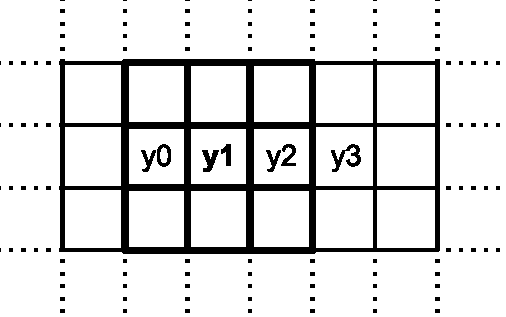
\includegraphics[scale=0.6]{figs/Stencil4.eps}
\end{center}
\caption{Overlapping support of four adjacent 3x3 stencils}
\label{fig:OverlappingSupport}
\end{figure}


% -----------------------------------------------------------------------------
\subsection{Cursored Arrays}
Recall the new Repa array representation from Figure \ref{fig:NewRepaArrays}. The definition of element generators is repeated below for reference. 

\begin{small}
\begin{code}
data Generator sh a
   = GenManifest { genVector :: Vector a }	
		
   | forall cursor. 
     GenCursored { genMake   :: sh -> cursor
                 , genShift  :: sh -> cursor -> cursor
                 , genLoad   :: cursor -> a }
\end{code}
\end{small}

A cursor is an abstract representation of an index into the array. The specific form of the cursor is defined by the \emph{producer} of the array, while the consumer must use the provided cursor functions to access elements. As hinted in the previous section, for stencil functions we represent the cursor by a linear index into the array. Given the coordinates of an element, @genMake@ computes the linear index of that element, the @genShift@ function shifts a cursor by an offset, and @genLoad@ produces the array element for a given cursor. Using cursors allows us to avoid repeated indexing computations like @x + y * width@, as we can now just compute the linear index of the centre of the stencil, then shift it around to get the other neighbouring elements.

As well as enabling sharing between index computations, cursored arrays strictly subsume our old delayed array representation. To see this, suppose we added an alternative to our @Generator@ type that implemented delayed arrays as given in \S\ref{sec:Repa}

\begin{small}
\begin{code}
  data Generator sh a
      = ...
      | GenDelayed { genGetElem  :: sh -> a }
\end{code}
\end{small}

It turns out this alternative is unnecessary, because we can write functions to convert between the delayed and cursored representations. Given a cursored array, we construct the element function for the delayed version making a cursor then immediately loading from it. Given a delayed array, we construct the cursored one by using the index itself as the cursor. This is possible due to the existential quantification of the @cursor@ type.

\begin{small}
\begin{code}
 delayedOfCursored :: Generator sh a -> Generator sh a
 delayedOfCursored (GenCursor make _ load)
         = GenDelayed (load . make)
 
 cursoredOfDelayed :: Generator sh a -> Generator sh a
 cursoredOfDelayed (GenDelayed getElem)
         = GenCursored id addIndex getElem

 addIndex :: Shape sh => sh -> sh -> sh
 addIndex = ...
\end{code}
\end{small}

To see that cursored arrays also support the delayed array approach to fusion, note that we can implement @map@ by composing its parameter with the @load@ function of the cursored array. The following code gives the definition of @mapGen@ which operates on the generator. The version for arrays is easily defined in terms of it.

\begin{small}
\begin{code}
 mapGen :: (a -> b) -> Generator sh a -> Generator sh b
 mapGen f gen
  = case arr of
     GenManifest vec  
       -> GenCursored id addDim  (\ix -> f (vec ! ix))
     GenCursored make shift load
       -> GenCursored make shift (f . load)
\end{code}
\end{small}

Finally, note that although we use cursored arrays internally to the library, there is usually no need for client programs to construct them explicitly. In the clients we have written, arrays are usually constructed with higher level utility functions, and combinators such as @map@ and @fold@ produce the same result independent of the representation of their arguments.

% -----------------------------------------------------------------------------
\subsection{Applying the Stencil}
\label{sec:ApplyingTheStencil}

% ----------------- FIG
\begin{figure}

\begin{small}
\begin{code}
data Boundary a
      = BoundConst a
      | BoundWrap
      | ...
	
mapStencil2 
  :: Boundary a -> Stencil DIM2 a
  -> Array DIM2 a -> Array DIM2 a

mapStencil2 boundary stencil@(Stencil sExtent _ _) arr
 = let (Z :. aHeight :. aWidth) = extent arr
       (Z :. sHeight :. sWidth) = sExtent

       rectsInternal    = ...
       rectsBorder      = ...
       inInternal ix    = ...
       inBorder   ix    = ...

       make  (Z:.y:.x)
        = Cursor (x + y*aWidth)
	
       shift (Z:.y:.x) (Cursor offset)
        = Cursor (offset + x + y*aWidth)

       loadBorder ix    = case boundary of ...
			
       loadInner cursor
        = unsafeAppStencil2 stencil arr shift cursor
							
   in  Array (extent arr)
        [ Region (RangeRects inBorder rectsBorder)
                 (GenCursored id addIndex loadBorder) 

        , Region (RangeRects inInternal rectsInternal)
                 (GenCursored make shift loadInner) ]


unsafeAppStencil2
  :: Stencil DIM2 a -> Array DIM2 a 
  -> (DIM2 -> Cursor -> Cursor)       -- shift cursor
  -> Cursor -> a

unsafeAppStencil2
  stencil@(Stencil sExtent sZero sAcc)
  arr@(Array aExtent [Region RangeAll (GenManifest vec)])
  shift cursor
 
  | _ :. sHeight :. sWidth  <- sExtent
  , sHeight <= 3, sWidth <= 3
  = template3x3 loadFromOffset sZero

  | otherwise = error "stencil too big for this method"

  where getData (Cursor index)
         = vec `unsafeIndex` index
		
        loadFromOffset oy ox	
         = let  offset = Z :. oy :. ox
                cur'   = shift offset cursor
           in   sAcc offset (getData cur')	


template3x3 :: (Int -> Int -> a -> a) -> a -> a
template3x3 f sZero
  =  f (-1) (-1)  $  f (-1)   0  $  f (-1)   1 
  $  f   0  (-1)  $  f   0    0  $  f   0    1   
  $  f   1  (-1)  $  f   1    0  $  f   1    1  
  $  sZero
\end{code}
\end{small}
\caption{Applying the stencil to an array}
\label{fig:MapStencil}
\end{figure}

Now that we have the definition for cursored arrays, we can see about creating one. Figure \ref{fig:MapStencil} gives the definition of @mapStencil2@ which takes the definition of a rank 2 stencil, a source array, and produces a cursored result array. The definitions of the rectangles for the border and internal regions have been elided to save space, as have the @inInternal@ and @inBorder@ predicates, though they are straightforward.

We have also elided the @INLINE@ pragmas for the @make@, @shift@ and @load@* functions. When compiling with GHC we must define these functions as separate bindings and give them @INLINE@ pragmas, instead of writing them as lambda abstractions directly in the body of the @let@ expression. Defining the functions this way ensures that when an array created with @mapStencil2@ is finally forced, these definitions are inlined into the unfolding of the @force@ function, as well as the element evaluation function @fillCursoredBlock2@ which we will discuss in the next section. If we do not do this, then the definitions would \emph{not} be appropriately inlined, and we would suffer a function call overhead for each application. We will return to this delicate point in \S\ref{sec:MultiStage}.

The values of the border elements depend on the @boundary@ parameter, and two options are shown at the top of the figure. The inner elements are defined via @unsafeAppStencil2@, which produces a function from the cursor value to the corresponding array element. Note that this function requires the provided source array to be manifest, so that elements can be extracted directly from the underling vector using @unsafeIndex@. We use @unsafeIndex@ to access the vector because this function performs no bounds checks, so we do not suffer the associated overhead. The safety of these accesses depends on the correctness of our library code, namely the @rectsInternal@ list from @mapStencil2@, so that @loadInner@ is not applied too close to the border.

Computation of the inner array elements is performed by the @loadFromOffset@ and @template3x3@ functions. The latter spells out every possible offset from the centre of a 3x3 stencil. We must spell out these offsets ``long hand'' instead of writing a recursive function to compute the result because we need each application of @f@ to be specialised for the provided offset. During compilation, @f@ will be bound to a coefficient function like the one defined in @laplace@ of Figure \ref{fig:NewSolveLaplace}. In effect, we are using @template3x3@ to select every possible coefficient that the coefficient function could have defined. By virtue of @makeStencil@ of Figure \ref{fig:Stencils}, if the coefficient function returns a valid coefficient for a particular offset then we end up with a term that multiplies that coefficient with data from the source array. If not, then the @Nothing@ branch of @makeStencil@ comes in to play and the result is unperturbed. Note that this mechanism permits us to use any stencil that \emph{fits inside} the 3x3 template. For example, stencils of size 3x1 and 2x2 also work.

Sadly, the fact that we must spell out every possible offset means that our @unsafeAppStencil2@ function is limited to handling stencils of a particular maximum size. In this case we have set the maximum to 3x3, so that it fits on the page. However, the limit is easy to increase and our concrete implementation currently uses 7x7. Limiting the size of the stencil in this way does not affect what coefficients or zero elements can be used, it just requires the entire stencil to fit inside the template. If we had instead written a recursive version of the template function, then GHC would not inline it, killing performance. In general, repeatedly inlining a recursive function may not terminate, leading to divergence at compile time. We can think of several ways of addressing this issue, but all require modification to the compiler, and we defer further discussion to \S\ref{sec:ManualUnwinding}. If the stencil does not fit inside the template then we fall back to the standard approach of loading the coefficients into a manifest array and iterating directly over that. This gets the job done, but obviously misses out on the benefits of the cursored approach. A follow on effect of spelling out every offset is that it also limits @mapStencil2@ to arrays of rank 2. It is straightforward to write versions for other ranks, as the general structure is the same as the rank-2 case, but we don't have a way of doing this polymorphically.

Finally, note that @unsafeAppStencil2@ defines a function between a cursor and a single array element. The task of actually filling the result array while exposing sharing between adjacent elements is performed by @fillCursoredBlock2@, which we discuss in the next section.


% -----------------------------------------------------------------------------
\subsection{Filling the Array, and Interaction with LLVM}
\label{sec:FillingTheArray}

% ----------------- FIG
\begin{figure}
\begin{small}
\begin{code}
case quotInt# ixLinear width  of { iX ->
case remInt#  ixLinear width  of { iY -> 
case +# iX (*# iY width) of { ixCenter ->
 writeFloatArray# world arrDest ixLinear
  (+##  (indexFloatArray# arrBV 
          (+# arrBV_start (+# (*# arrBV_width iY) iX)))
   (*## (indexFloatArray# arrBM 
          (+# arrBM_mask  (+# (*# arrBM_width iY) iX)))
    (/## (+## (+## (+##
      (indexFloatArray# arrSrc 
       (+# arrSrc_start (+# ixCenter width)))
      (indexFloatArray# arrSrc
       (+# arrSrc_start (+# ixCenter 1))))
      (indexFloatArray# arrSrc
       (+# arrSrc_start (+# ixCenter (-1)))))
      (indexFloatArray# arrSrc
       (+# arrSrc_start (+# ixCenter (*# (-1) width)))))
     4.0))) }}
\end{code}
\end{small}
\caption{New core IR for Laplace with index sharing}
\label{fig:NewLaplaceIndexCore}
\end{figure}


% ----------------- FIG
\begin{figure}
\begin{small}
\begin{code}
fillCursoredBlock2
 :: IOVector a                   -- vector to write into
 -> (DIM2   -> cursor)           -- makeCursor
 -> (DIM2   -> cursor -> cursor) -- shiftCursor
 -> (cursor -> a) -> Int         -- loadElem, width
 -> Int -> Int -> Int -> Int     -- coords of block
 -> IO ()
fillCursoredBlock2 !vec !make !shift !load
   !width !x0 !y0 !x1 !y1 = ... fillRow4 ...
 where 
    fillRow4 !y !x    -- fill a single row in the block
     | x + 4 > x1     = ... -- less than 4 elems remaining
     | otherwise
     = do let srcCur0 = make  (Z:.y:.x)
          let srcCur1 = shift (Z:.0:.1) srcCur0
          let srcCur2 = shift (Z:.0:.1) srcCur1
          let srcCur3 = shift (Z:.0:.1) srcCur2

          let val0    = load srcCur0
          let val1    = load srcCur1
          let val2    = load srcCur2
          let val3    = load srcCur3
          touch val0; touch val1; touch val2; touch val3

          let !dstCur0 = x + y * width
          unsafeWrite vec (dstCur0)     val0
          unsafeWrite vec (dstCur0 + 1) val1
          unsafeWrite vec (dstCur0 + 2) val2
          unsafeWrite vec (dstCur0 + 3) val3
          fillRow4 y (x + 4)
\end{code}	
\end{small}
\caption{Block evaluation function for cursored DIM2 arrays}
\label{fig:BlockEvaluation}
\end{figure}

Using our original @force@ function (not shown), but with cursored arrays, produces a loop whose inner fragment consists of the Core IR shown in Figure \ref{fig:NewLaplaceIndexCore}. The loop as a whole iterates through the linear indices of the result vector. In the body, each linear index (@ixLinear@) is converted to a rank-2 index, then back to a cursor value @ixCenter@. As the source and destination arrays have the same dimensions, @ixLinear@ and @ixCenter@ will have the same value. The intermediate conversion is successfully eliminated by the LLVM optimiser, so doesn't appear in the object code. 

Note how each of the elements of the source array are indexed relative to the cursor @ixCenter@. To recover sharing between adjacent elements we must evaluate several in the same iteration, which requires a new version of @force@. The inner loop of this new version is defined by @fillCursoredBlock2@ in Figure \ref{fig:BlockEvaluation}, which is also part of the library. This function takes a mutable @IOVector@, along with the functions that form a cursored array, and uses them to fill a rectangular block in the vector. Parallelism is introduced by having @force@ fork off several threads, with each filling a different block of array elements. Performing block-wise evaluation also improves cache usage, as the evaluation of each successive row in a block usually requires source elements that were loaded into cache during the evaluation of previous rows.

In the definition of @fillCursoredBlock2@ we have manually applied the \mbox{\emph{unroll-and-jam}} transformation \cite{Carr:unroll-and-jam} to evaluate groups of four consecutive elements per iteration. We operate row-wise, which is good for regions that are at least four elements wide. To evaluate narrow regions such as the one pixel wide left-hand border from Figure \ref{fig:StencilBorder} it is better to operate column-wise, using a separate filling function derived from the presented code.

The @touch@ function in the inner loop is used to place a dependency on the computed array values, and prevent GHC from floating the @srcCur@* and @val@* bindings into the applications of @unsafeWrite@. The @touch@ function has the following type, and is defined in terms of the GHC primitive operation @touch#@. 

\begin{small}
\begin{code}
  touch :: Elt a => a -> IO ()
\end{code}
\end{small}

We need all four element values to be computed \emph{before} any of them are written to the result array. This is to avoid a hairy interaction with the LLVM optimiser. Specifically, LLVM does not know that the low-level representation of the source and result arrays do not alias, nor does it know that the result array and GHC \emph{stack} do not alias. Any write to the result array or stack is assumed to also modify the source array, which invalidates data held in registers at that point. This in turn breaks the GVN (Global Value Numbering) optimisation which we depend on to recover sharing.

The disassembled x86\_64 object code for the inner part of our loop is given in Figure \ref{fig:SobelAssembly}. This is for the $Sobel_X$ stencil shown in Figure \ref{Fig:ExampleKernels}. Floating point loads are marked with round bullets, while floating point stores are marked with diamonds. There are 18 loads and 4 stores, and examining Figure \ref{fig:OverlappingSupport} shows that this is the optimal number for such a 3x3 stencil. However, we still have a slight inefficiency due to aliasing issues. Note the repeated instruction @mov 0x6(rbx),rcx@ after each floating point store. The @rbx@ register contains a pointer to the stack, and each floating point store invalidates the previously loaded value in @rcx@. Aliasing becomes more of a problem when compiling to architectures with insufficient floating point registers. For example 32bit x86 code can only address 8 of the 16 XMM registers available in 64bit mode. If the LLVM compiler runs out of registers then it spills values to the stack, which also invalidates previously loaded values. Fixing this will require more work on GHC's LLVM backend, and/or a type system or analysis that recovers the non-aliasing of heap objects.

Finally, note that the optimal number of elements to compute per iteration depends on the form of the stencil, namely how many coefficients overlap when several stencils are placed side-by-side. Computing too few elements per iteration limits how much sharing can be recovered, while computing too many increases register pressure and can cause intermediate values to be spilled to the stack. Currently, we always compute four at once, which works well for most 3x3 stencils. In future work we intend to add a size-hint to our @Array@ type, which would be set by @mapStencil2@. The @fillCursoredBlock2@ function would use this hint to choose between several loops, all with the same form as @fillRow4@, but computing a different number of elements per iteration.


% ------------------------------------- FIG

% Macros for formatting assembly code.
\newcommand{\asm}[3]	
{		& \hspace{-2em} {\tt #1:} 
		& \hspace{-2em} {\tt #2} 
		& \hspace{-1em} {\tt #3} \\}

\newcommand{\aasm}[4]
{\hspace{-1em} #1 \hspace{-3em}  
		& \hspace{-2em} {\tt #2:}
		& \hspace{-2em} {\tt #3}
		& \hspace{-1em} {\tt #4} \\}

\newcommand{\lasm}[3]	{ \aasm{$\bullet$}	{#1}{#2}{#3} }
\newcommand{\sasm}[3]	{ \aasm{$\diamond$}	{#1}{#2}{#3} }


\begin{figure}
\begin{minipage}[b]{0.5\linewidth}
\begin{tiny}
\begin{tabular}{lrll}
\asm	{9b0}	{mov}	{0x2e(rbx), rcx}
\asm	{9b4}	{mov}	{0x1e(rbx), rdx}
\asm	{9b8}	{mov}	{rdx, rsi}
\asm	{9bb}	{imul}	{rcx, rsi}
\asm	{9bf}	{mov}   {0x36(rbx), rdi}
\asm	{9c3}	{lea}   {0x4(r14,rdi,1), r8}
\asm	{9c8}	{add}   {r14, rdi}
\asm	{9cb}	{lea}   {0x1(rcx), r9}
\asm	{9cf}	{imul}  {rdx, r9}
\asm	{9d3}	{lea}   {0x2(r9,rdi,1), r10}
\asm	{9d8}	{mov}   {0x6(rbx), r11}
\asm	{9dc}	{mov}   {0xe(rbx), r15}
\\
\lasm 	{9e0}	{movss} {0x10(r15,r10,4), xmm7}
\asm	{9e7}	{lea}   {(r8,r9,1), r10}
\lasm	{9eb}	{movss} {0x10(r15,r10,4), xmm8}
\asm	{9f2}	{subss} {xmm7, xmm8}
\asm	{9f7}	{lea}   {(r8,rsi,1), r10}
\lasm	{9fb}	{movss} {0x10(r15,r10,4), xmm9}
\asm	{a02}	{addss} {xmm9, xmm9}
\asm	{a07}	{addss} {xmm8, xmm9}
\asm	{a0c}	{lea}   {0x2(rsi,rdi,1), r10}
\lasm	{a11}	{movss} {0x10(r15,r10,4), xmm8}
\asm	{a18}	{movaps}{xmm8, xmm10}
\asm	{a1c}	{mulss} {xmm0, xmm10}
\asm	{a21}	{addss} {xmm9, xmm10}
\asm	{a26}	{dec}   {rcx}
\asm	{a29}	{imul}  {rdx,rcx}
\asm	{a2d}	{add}   {rcx,r8}
\\
\lasm	{a30}	{addss} {0x10(r15,r8,4), xmm10}
\asm	{a37}	{lea}   {0x1(r9,rdi,1), rdx}
\lasm	{a3c}	{movss} {0x10(r15,rdx,4), xmm9}
\asm	{a43}	{lea}   {0x3(r9,rdi,1), rdx}
\lasm	{a48}	{movss} {0x10(r15,rdx,4), xmm11}
\asm	{a4f}	{subss} {xmm9, xmm11}
\asm	{a54}	{lea}   {0x3(rsi,rdi,1), rdx}
\lasm	{a59}	{movss} {0x10(r15,rdx,4), xmm12}
\asm	{a60}	{addss} {xmm12, xmm12}
\asm	{a65}	{addss} {xmm11, xmm12}
\asm	{a6a}	{lea}   {0x1(rsi,rdi,1), rdx}
\lasm	{a6f}	{movss} {0x10(r15,rdx,4), xmm11}
\asm	{a76}	{movaps}{xmm11, xmm13}
\asm	{a7a}	{mulss} {xmm0, xmm13}
\asm	{a7f}	{addss} {xmm12, xmm13}
\asm	{a84}	{lea}   {0x3(rcx,rdi,1), rdx}
\lasm	{a89}	{addss} {0x10(r15,rdx,4), xmm13}
\\
\end{tabular}
\end{tiny}
\end{minipage}
% --------------------
\begin{minipage}[b]{0.5\linewidth}
\begin{tiny}
\begin{tabular}{lrll}
\asm	{a90}	{lea}	{(rdi,r9,1), rdx}
\lasm	{a94}	{subss}	{0x10(r15,rdx,4), xmm7}
\asm	{a9b}	{addss}	{xmm8, xmm8}
\asm	{aa0}	{addss}	{xmm7, xmm8}
\asm	{aa5}	{lea}	{0x1(rcx,rdi,1), rdx}
\asm	{aaa}	{lea}	{0x2(rcx,rdi,1), r8}
\asm	{aaf}	{lea}	{(rdi,rsi,1), r10}
\lasm	{ab3}	{movss}	{0x10(r15,r10,4), xmm7}
\asm	{aba}	{mulss}	{xmm0, xmm7}
\asm	{abe}	{addss}	{xmm8, xmm7}
\lasm	{ac3}	{movss}	{0x10(r15,r8,4), xmm8}
\asm	{aca}	{addss}	{xmm8, xmm7}
\asm	{acf}	{lea}	{(rdi,rcx,1), r8}
\lasm	{ad3}	{subss}	{0x10(r15,r8,4), xmm7}
\\
\asm	{ada}	{add}   {rax, rdi}
\asm	{add}	{add}   {rdi, r9}
\lasm	{ae0}	{subss} {0x10(r15,r9,4), xmm9}
\asm	{ae7}	{addss} {xmm11, xmm11}
\asm	{aec}	{addss} {xmm9, xmm11}
\asm	{af1}	{lea}   {(rdi,rsi,1), r8}
\lasm	{af5}	{movss} {0x10(r15,r8,4), xmm9}
\asm	{afc}	{mulss} {xmm0, xmm9}
\asm	{b01}	{addss} {xmm11, xmm9}
\lasm	{b06}	{movss} {0x10(r15,rdx,4), xmm11}
\asm	{b0d}	{addss} {xmm11, xmm9}
\asm	{b12}	{add}   {rcx, rdi}
\lasm	{b15}	{subss} {0x10(r15,rdi,4), xmm9}
\\
\asm	{b1c}	{add}   {r14,rsi}
\sasm	{b1f}	{movss} {xmm9,0x10(r11,rsi,4)}
\asm	{b26}	{mov}   {0x6(rbx),rcx}
\sasm	{b2a}	{movss} {xmm7,0x14(rcx,rsi,4)}
\asm	{b30}	{subss} {xmm11,xmm13}
\asm	{b35}	{mov}   {0x6(rbx),rcx}
\sasm	{b39}	{movss} {xmm13,0x18(rcx,rsi,4)}
\asm	{b40}	{subss} {xmm8,xmm10}
\asm	{b45}	{mov}   {0x6(rbx),rcx}
\sasm	{b49}	{movss} {xmm10,0x1c(rcx,rsi,4)}
\asm	{b50}	{lea}   {0x8(r14),rcx}
\asm	{b54}	{lea}   {0x4(r14),r14}
\asm	{b58}	{cmp}   {0x26(rbx),rcx}
\asm	{b5c}	{jle}   {9b0}
\end{tabular}
\end{tiny}
\end{minipage}

\caption
	{ x86\_64 assembly for $Sobel_X$  applied to four consecutive pixels. 
	  FP loads and stores are marked with $\bullet$ and $\diamond$. }
\label{fig:SobelAssembly}
\end{figure}



